\documentclass[]{article}
\usepackage[T1]{fontenc}
\usepackage{lmodern}
\usepackage{amssymb,amsmath}
\usepackage{ifxetex,ifluatex}
\usepackage{fixltx2e} % provides \textsubscript
% use upquote if available, for straight quotes in verbatim environments
\IfFileExists{upquote.sty}{\usepackage{upquote}}{}
\ifnum 0\ifxetex 1\fi\ifluatex 1\fi=0 % if pdftex
  \usepackage[utf8]{inputenc}
\else % if luatex or xelatex
  \ifxetex
    \usepackage{mathspec}
    \usepackage{xltxtra,xunicode}
  \else
    \usepackage{fontspec}
  \fi
  \defaultfontfeatures{Mapping=tex-text,Scale=MatchLowercase}
  \newcommand{\euro}{€}
\fi
% use microtype if available
\IfFileExists{microtype.sty}{\usepackage{microtype}}{}
\usepackage[margin=1in]{geometry}
\usepackage{color}
\usepackage{fancyvrb}
\newcommand{\VerbBar}{|}
\newcommand{\VERB}{\Verb[commandchars=\\\{\}]}
\DefineVerbatimEnvironment{Highlighting}{Verbatim}{commandchars=\\\{\}}
% Add ',fontsize=\small' for more characters per line
\usepackage{framed}
\definecolor{shadecolor}{RGB}{248,248,248}
\newenvironment{Shaded}{\begin{snugshade}}{\end{snugshade}}
\newcommand{\KeywordTok}[1]{\textcolor[rgb]{0.13,0.29,0.53}{\textbf{{#1}}}}
\newcommand{\DataTypeTok}[1]{\textcolor[rgb]{0.13,0.29,0.53}{{#1}}}
\newcommand{\DecValTok}[1]{\textcolor[rgb]{0.00,0.00,0.81}{{#1}}}
\newcommand{\BaseNTok}[1]{\textcolor[rgb]{0.00,0.00,0.81}{{#1}}}
\newcommand{\FloatTok}[1]{\textcolor[rgb]{0.00,0.00,0.81}{{#1}}}
\newcommand{\CharTok}[1]{\textcolor[rgb]{0.31,0.60,0.02}{{#1}}}
\newcommand{\StringTok}[1]{\textcolor[rgb]{0.31,0.60,0.02}{{#1}}}
\newcommand{\CommentTok}[1]{\textcolor[rgb]{0.56,0.35,0.01}{\textit{{#1}}}}
\newcommand{\OtherTok}[1]{\textcolor[rgb]{0.56,0.35,0.01}{{#1}}}
\newcommand{\AlertTok}[1]{\textcolor[rgb]{0.94,0.16,0.16}{{#1}}}
\newcommand{\FunctionTok}[1]{\textcolor[rgb]{0.00,0.00,0.00}{{#1}}}
\newcommand{\RegionMarkerTok}[1]{{#1}}
\newcommand{\ErrorTok}[1]{\textbf{{#1}}}
\newcommand{\NormalTok}[1]{{#1}}
\usepackage{graphicx}
% Redefine \includegraphics so that, unless explicit options are
% given, the image width will not exceed the width of the page.
% Images get their normal width if they fit onto the page, but
% are scaled down if they would overflow the margins.
\makeatletter
\def\ScaleIfNeeded{%
  \ifdim\Gin@nat@width>\linewidth
    \linewidth
  \else
    \Gin@nat@width
  \fi
}
\makeatother
\let\Oldincludegraphics\includegraphics
{%
 \catcode`\@=11\relax%
 \gdef\includegraphics{\@ifnextchar[{\Oldincludegraphics}{\Oldincludegraphics[width=\ScaleIfNeeded]}}%
}%
\ifxetex
  \usepackage[setpagesize=false, % page size defined by xetex
              unicode=false, % unicode breaks when used with xetex
              xetex]{hyperref}
\else
  \usepackage[unicode=true]{hyperref}
\fi
\hypersetup{breaklinks=true,
            bookmarks=true,
            pdfauthor={Víctor Funes Leal},
            pdftitle={Trabajo Práctico-Evalución de Impacto de Políticas Públicas 2014},
            colorlinks=true,
            citecolor=blue,
            urlcolor=blue,
            linkcolor=magenta,
            pdfborder={0 0 0}}
\urlstyle{same}  % don't use monospace font for urls
\setlength{\parindent}{0pt}
\setlength{\parskip}{6pt plus 2pt minus 1pt}
\setlength{\emergencystretch}{3em}  % prevent overfull lines
\setcounter{secnumdepth}{0}

\title{Trabajo Práctico-Evalución de Impacto de Políticas Públicas 2014}
\author{Víctor Funes Leal}
\date{}

\begin{document}

\begin{center}
\huge Trabajo Práctico-Evalución de Impacto de Políticas Públicas 2014 \\[0.2cm]
\large \emph{Víctor Funes Leal}\\[0.1cm]
\normalsize
\end{center}


{
\hypersetup{linkcolor=black}
\setcounter{tocdepth}{2}
\tableofcontents
}
\newpage

\section{Detalles de la simulación}\label{detalles-de-la-simulacion}

\subsection{Modelo utilizado}\label{modelo-utilizado}

El presente trabajo práctico busca replicar los resultados de Heckman,
Lalonde y Smith (1999)(Heckman, Lalonde, and Smith 1999), quienes
afirman que los modelos de evaluación de impacto de políticas públicas
poseen dos elementos:

\begin{enumerate}
\def\labelenumi{\arabic{enumi}.}
\itemsep1pt\parskip0pt\parsep0pt
\item
  El modelo de la variable de resultado
\item
  El modelo para la participación en el programa
\end{enumerate}

La estructura que se utiliza en este trabajo (y que utilizan los
autores) puede describirse por medio de las siguientes ecuaciones:

\[ Y_{it}=\beta+\alpha_{i}D_{i}+\theta_{i}+U_{it} \] si $t>k$.
\[ Y_{it}=\beta+\theta_{i}+U_{it} \] si $t<k$.
\[ U_{it}=\rho U_{it-1}+\epsilon_{it}\]

En donde $Y_{it}$ es el ingreso de los individuos, $\beta$ es una forma
de ingreso permanente, $\alpha_{i}$ es el efecto del programa para
quienes acceden a él, $\theta_{i}$ es un efecto fijo individual no
observable. Por su parte el componente no observable posee una parte que
evoluciona como un proceso estcástico autoregresivo de orden 1 cuyo
coeficiente de autocorrelación está dado por el parámetro $\rho$, a su
vez éste componente no observable posee un shock aleatorio contemporáneo
$\epsilon_{it}$.

El entrenamiento tiene lugar en el año $k$ y los individuos que deciden
participar de éste los que la variable dummy $D_{i}$ es igual a uno. La
decisión de participar depende del valor actual esperado de los
beneficios futuros ($\alpha_{i}/r$, dónde $r$ es la tasa de descuento),
del ingreso que se renuncia en el año que accede al programa de
entrenamiento $Y_{ik}$ y de un costo idiosincrático específico a cada
individuo $c_{i}$ que se interpreta como la matrícula que debe pagar (en
el caso que sea positivo) o el subsidio que recibe para participar (en
el caso que sea negativo) y que se describe por medio de la fórmula:
$c_{i}=\Phi Z_{i}+V_{i}$, dónde $Z_{i}$ y $V_{i}$ son variables
aleatorias independientes entre sí y de las demás.

\[ D_{i}=\begin{cases} 1 & \alpha_{i}/r-Y_{ik}-c_{i}>0\text{ y }t>k\\ 0 & \text{ caso contrario}\end{cases} \]

\subsection{Proceso generador de
datos}\label{proceso-generador-de-datos}

Para el ejercicio de simulación se utilizan las siguientes variables y
distribuciones:

\begin{itemize}
\itemsep1pt\parskip0pt\parsep0pt
\item
  Existen 1000 individuos para los que se simulan 10 años de datos de
  ingresos y a su vez, se replican 100 muestras.
\item
  Los 10 años se distribuyen de la sigueinte forma: hay 5 años pre
  programa ($k-5$ a $k-1$), un año de implementación ($k=6$) y cuatro
  años post programa ($k+1$ a $k+4$).
\item
  El ingreso permanente es igual para todos los individuos
  ($\beta=1000$).
\item
  El efecto tratamiento ($\alpha_{i}$) se distribuye como normal con
  media 100 y desv. estándar igual a 300: $\alpha_{i}\sim N(100,300)$.
\item
  El efecto fijo también se distribuye de la misma forma con media 0 y
  desv. estándar igual a 300: $\alpha_{i}\sim N(100,300)$.
\item
  El componente idiosincrático de error se distribuye también como
  normal con media igual a 0 y desv. estándar igual a 280:
  $\epsilon_{it}\sim N(100,280)$.
\item
  Se supone que $U_{ik-5}=\epsilon_{ik-5}$ y que $\rho=0,78$.
\item
  Por último los componentes de la función de costos se distribuyen como
  normales con $\Phi=1$, $V_{i}\sim N(100,200)$ y
  $Z_{i}\sim N(\mu_{Z},200)$, dónde $\mu_{Z}$ se escoge de manera tal
  que para todas las muestras el 10\% de la población participe del
  programa y la tasa de interés ($r$) es igual a 0,10.
\end{itemize}

\subsection{Carga de los parámetros}\label{carga-de-los-parametros}

En primer lugar, el programa requiere que se fijen valores para todos
los parámetros, según lo indicado en el punto anterior:

\begin{Shaded}
\begin{Highlighting}[]
\NormalTok{n<-}\DecValTok{1000}
\NormalTok{beta<-}\KeywordTok{rep}\NormalTok{(}\DecValTok{1000}\NormalTok{,n)}
\NormalTok{r<-}\FloatTok{0.1}
\NormalTok{rho<-}\StringTok{ }\FloatTok{0.78}
\NormalTok{phi<-}\DecValTok{1}
\NormalTok{mean_alpha<-}\DecValTok{100}
\NormalTok{sd_alpha<-}\DecValTok{300} \CommentTok{#(=0 para el modelo de coeficientes comunes, =300 para coef. aleatorios)}
\NormalTok{mean_theta<-}\DecValTok{0}
\NormalTok{sd_theta<-}\DecValTok{300}
\NormalTok{mean_epsilon<-}\DecValTok{0}
\NormalTok{sd_epsilon<-}\DecValTok{280}
\NormalTok{mean_v<-}\DecValTok{0}
\NormalTok{sd_v<-}\DecValTok{200}
\NormalTok{sd_z<-}\DecValTok{300}
\end{Highlighting}
\end{Shaded}

El comando \texttt{rep} replica el valor de $\beta$ (1000) $n$ veces, en
esta caso también igual a 1000 con el objeto de agregarlo posteriormente
a los vectores de ingresos.

Luego, se generan las variables aletorias tambén detalladas previamente:

\begin{Shaded}
\begin{Highlighting}[]
\CommentTok{#Generar variables aleatorias}
\NormalTok{alpha_i<-}\KeywordTok{rnorm}\NormalTok{(n, mean_alpha, sd_alpha)}
\NormalTok{theta_i<-}\KeywordTok{rnorm}\NormalTok{(n, mean_theta, sd_theta)}
\NormalTok{V_i<-}\KeywordTok{rnorm}\NormalTok{(n, mean_v, sd_v)}
\NormalTok{Epsilon_it<-}\KeywordTok{replicate}\NormalTok{(}\DecValTok{10}\NormalTok{, }\KeywordTok{rnorm}\NormalTok{(n, mean_epsilon, sd_epsilon)) }
\end{Highlighting}
\end{Shaded}

Las variables aleatorias $\alpha_{i}$, $\theta_{i}$ y $V_{i}$ se crean
con una funcion \texttt{rnorm} que genera $n$ números aletorios
normalmente distribuidos cuya media es el valor que corresponde al
segundo argumaneto y su desviación estándar es igual al tercero. Los
valores de $\epsilon_{it}$ deben ser distintos apra cada uno de los 10
años, por lo que se generó una matriz de $1000\times 10$ (1000
individuos en 10 años) de numeros aleatorios normales con media y
desviación estándar detalladas, para ello se utilizó el comando
\emph{replicate} que, justamente, replica el vector de 1000 número
aleatorios 10 veces, generando cada vez una realización distinta.

Para los valores del término aleatorio $U_{it}$ y para los ingresos
$Y_{it}$ se optó por la siguiente estrategia: crear dos matrices de
$1000\times 10$ dónde cada columna es uno de los 10 años en los que se
simula la intervención y cada fila es uno de los 1000 individuos que
forman parte del estudio.

\begin{Shaded}
\begin{Highlighting}[]
\CommentTok{#Generar data frame para guardar los datos}
\NormalTok{dat<-}\KeywordTok{data.frame}\NormalTok{(}\KeywordTok{matrix}\NormalTok{(}\DecValTok{0}\NormalTok{, }\DataTypeTok{ncol=}\DecValTok{10}\NormalTok{, }\DataTypeTok{nrow=}\NormalTok{n))}

\CommentTok{#Nombres de las 10 columnas de la matriz de ingresos}
\NormalTok{y<-}\KeywordTok{rep}\NormalTok{(}\DecValTok{0}\NormalTok{,}\DecValTok{10}\NormalTok{)}
\NormalTok{for(i in }\DecValTok{1}\NormalTok{:}\DecValTok{10}\NormalTok{)\{}
  \NormalTok{y[i]<-}\KeywordTok{paste}\NormalTok{(}\StringTok{"y_"}\NormalTok{,i, }\DataTypeTok{sep=}\StringTok{""}\NormalTok{)}
\NormalTok{\}}
\KeywordTok{colnames}\NormalTok{(dat)<-y}
\end{Highlighting}
\end{Shaded}

En primer lugar se genera una matriz ``vacía'' de dimensiones
$1000\times 10$ (en realidad con todos sus elementos iguales a cero) y
luego se colocan los nombres de las columnas con un bucle, de manera tla
que sean iguales a $Y_i$ con $i=1\dots,10$.

De idéntica manera se crea la matriz \texttt{Ui\_t}, la cual posee la
particularidad que sus columnas dependen de los valores de la matriz
\texttt{Epsilon\_it}, la primer columna de ambas matrices es igual, pero
de la columna 2 en adelante se crean según la fórmula del proceso AR(1).

\begin{Shaded}
\begin{Highlighting}[]
\NormalTok{U_it<-}\KeywordTok{matrix}\NormalTok{(}\DecValTok{0}\NormalTok{, }\DataTypeTok{nrow=}\NormalTok{n, }\DataTypeTok{ncol=}\DecValTok{10}\NormalTok{)}
\NormalTok{U_it[,}\DecValTok{1}\NormalTok{]=Epsilon_it[,}\DecValTok{1}\NormalTok{]}

\NormalTok{for(k in }\DecValTok{2}\NormalTok{:}\DecValTok{10}\NormalTok{)\{}
  \NormalTok{U_it[,k]=rho*U_it[,k}\DecValTok{-1}\NormalTok{]+Epsilon_it[,k]}
\NormalTok{\}}
\end{Highlighting}
\end{Shaded}

Luego se procede a rellenar los valores de la matriz de ingresos
(\texttt{dat}), para ello se requieren valores para $D_{i}$ pero, dado
que para los períodos 1 a 6 nadie participa porque todavía no se
implementó el programa, son iguales a cero para todos los individuos.

\begin{Shaded}
\begin{Highlighting}[]
\CommentTok{#Período incial}
\CommentTok{#Nadie participa antes de la implementación del programa}
\NormalTok{D_i<-}\KeywordTok{rep}\NormalTok{(}\DecValTok{0}\NormalTok{, n)}
\NormalTok{dat[,}\DecValTok{1}\NormalTok{]<-beta+alpha_i*D_i+theta_i+U_it[,}\DecValTok{1}\NormalTok{]}

\CommentTok{#Períodos 2 a 5: se generan los ingresos según la ley de movimiento de U_it}
\NormalTok{for(k in }\DecValTok{2}\NormalTok{:}\DecValTok{5}\NormalTok{)\{}
  \NormalTok{dat[,k]<-beta+alpha_i*D_i+theta_i+U_it[,k]}
\NormalTok{\}}
\end{Highlighting}
\end{Shaded}

En el período 6 se implementa el programa y, como primera medida, debe
individualizarse a quienes participan de los que no por medio de la
variable $D_{i}$, éste valor dependerá de la media de la variable
aleatoria $Z_{i}$, la cual debe fijarse de manera tal que para cada
muestra participe el 10\% de los individuos. Ésto se logró por medio de
un bucle que itera hasta que se cumple la condición especificada, ahora
bien, la velocidad de convergencia depende del valor inicial, elcual,
tras varias pruebas se fijó en 700 para el modelo de coeficientes coumes
($\alpha_{i}=\alpha\, \forall i$) y en 4000 para el modelo de
coeficientes aleatorios.

\begin{Shaded}
\begin{Highlighting}[]
\CommentTok{#mu<-700 Coeficientes comunes}
\NormalTok{mu<-}\DecValTok{4000} \CommentTok{#Coeficientes aleatorios}
\NormalTok{ntreated<-}\DecValTok{0}
\NormalTok{y<-beta+alpha_i*D_i+theta_i+U_it[,}\DecValTok{6}\NormalTok{]}
\NormalTok{while(ntreated!=}\DecValTok{100}\NormalTok{)\{}
  \NormalTok{Z_i<-}\KeywordTok{rnorm}\NormalTok{(n, mu, sd_z)}
  \NormalTok{c_i<-Z_i*phi+V_i}
  \NormalTok{D_i<-}\KeywordTok{as.numeric}\NormalTok{(}\KeywordTok{I}\NormalTok{((alpha_i/r-y-c_i)>}\DecValTok{0}\NormalTok{))}
  \NormalTok{ntreated<-}\KeywordTok{as.numeric}\NormalTok{(}\KeywordTok{table}\NormalTok{(D_i)[}\DecValTok{2}\NormalTok{])}
  \CommentTok{#si participantes < 1000 reduce la media de u, caso contrario la aumenta}
  \NormalTok{if(ntreated<}\DecValTok{100}\NormalTok{)\{}
    \NormalTok{mu=mu}\DecValTok{-1}
  \NormalTok{\}else\{}
    \NormalTok{mu=mu}\DecValTok{+1}
  \NormalTok{\}}
\NormalTok{\}}
  \KeywordTok{print}\NormalTok{(}\KeywordTok{paste}\NormalTok{(}\StringTok{"Media de u: "}\NormalTok{, mu))}
\end{Highlighting}
\end{Shaded}

\begin{verbatim}
## [1] "Media de u:  4100"
\end{verbatim}

\begin{Shaded}
\begin{Highlighting}[]
  \KeywordTok{print}\NormalTok{(}\KeywordTok{paste}\NormalTok{(}\StringTok{"Número de participantes: "}\NormalTok{, ntreated))  }
\end{Highlighting}
\end{Shaded}

\begin{verbatim}
## [1] "Número de participantes:  100"
\end{verbatim}

El algoritmo converge rápidamente al valor de 100 individuos, a partir
de los cuales se genera el vector $D_{i}$ que indica cuáles de ellos
participan del programa y cuales no.

Luego se rellenan los valores del período 6 haciendo que $Y_{ik}=0$ si
$D_{i}=1$ (quienes participan no obtienen ingresos en el período),
mientras que los que no participan continuán generando sus ingreos según
la misma ley de movimiento. Por último, para los períodos 7 a 10 se
vuelve al esquema anterior, pero partiendo de los nuevos valores de
$D_{i}$ iguales a 1 para 100 perosnas y cero apra los 900 remanentes.

\begin{Shaded}
\begin{Highlighting}[]
\CommentTok{#Reemplazo valores para el período 6 (0 para los que participan)}
\NormalTok{dat[,}\DecValTok{6}\NormalTok{]<-(}\DecValTok{1}\NormalTok{-D_i)*(beta+alpha_i+theta_i+U_it[,}\DecValTok{6}\NormalTok{])}


\CommentTok{#Períodos 7 a 10: se generan los ingresos según la ley de movimiento}
\NormalTok{for(k in }\DecValTok{7}\NormalTok{:}\DecValTok{10}\NormalTok{)\{}
  \NormalTok{dat[,k]<-beta+alpha_i*D_i+theta_i+U_it[,k]}
\NormalTok{\}}
\end{Highlighting}
\end{Shaded}

Una vez creada la matriz de valores puede observarse su composición por
medio de los valores de los primeros 6 individuos a través del comando
\texttt{head}:

\begin{Shaded}
\begin{Highlighting}[]
\KeywordTok{head}\NormalTok{(dat)}
\end{Highlighting}
\end{Shaded}

\begin{verbatim}
##      y_1    y_2     y_3    y_4    y_5    y_6    y_7    y_8    y_9   y_10
## 1  302.7 -201.8  -66.73  384.8  590.9  114.5  436.0  576.2  300.7  636.1
## 2 1451.6 1138.1 1264.00 1107.4  892.4  546.7  865.4  480.1 1074.4  442.3
## 3  669.5  627.3  335.75  174.3  428.4  783.0  939.4 1550.0 1873.2 1558.3
## 4 1010.7 1426.5 1869.04 1720.8 1458.3 1983.0 1937.1 2179.5 2189.8 2098.8
## 5 1772.1 1663.4 1920.37 1100.4 1462.7 1212.5 1268.9  805.4  589.4  754.9
## 6 1414.3 1389.5 1388.51 1512.9 1408.6 1526.1 1432.5 1604.0 2095.7 2097.3
\end{verbatim}

Y luego, se agregan las columnas de valores de $\alpha_{i}$ y $D_{i}$ a
la matriz de datos, puesto que se los requerirá posteriormente.

\begin{Shaded}
\begin{Highlighting}[]
\NormalTok{dat<-}\KeywordTok{cbind}\NormalTok{(dat, alpha_i, D_i)}
\end{Highlighting}
\end{Shaded}

\section{Matching}\label{matching}

Ahora se utiliza un estimador de ``matching'' con el objeto de aparear
observaciones entre los 100 individuos del grupo de tratamiento y un
subconjunto de individuos del grupo de contol. En este caso el
apareamiento se realiza por el criterio del ``vecino más cercano''
(nearest neighbour) con reemplazo.

Para realizar el mencionado análisis se utilizó la librería
``MatchIt''(Ho et al. 2011), la cual posee un comando para aparear datos
(\texttt{matchit}), utilizando diversos métodos de matching (exacto,
genético, vecino más cercano, óptimo, etc.) y permitiendo también
escoger la función de distancia a utilizar, en este caso se optó por la
función logística, además, se incluye la opción \texttt{replace=TRUE}
para que el apareamiento sea con reemplazo.

\begin{Shaded}
\begin{Highlighting}[]
\KeywordTok{library}\NormalTok{(MatchIt)}
\end{Highlighting}
\end{Shaded}

\begin{verbatim}
## Loading required package: MASS
\end{verbatim}

\begin{Shaded}
\begin{Highlighting}[]
\NormalTok{match<-}\KeywordTok{matchit}\NormalTok{(D_i~y_4, }\DataTypeTok{method=}\StringTok{"nearest"}\NormalTok{, }\DataTypeTok{distance=}\StringTok{"logit"}\NormalTok{, }\DataTypeTok{data=}\NormalTok{dat, }\DataTypeTok{replace=}\OtherTok{TRUE}\NormalTok{)}
\KeywordTok{summary}\NormalTok{(match)}
\end{Highlighting}
\end{Shaded}

\begin{verbatim}
## 
## Call:
## matchit(formula = D_i ~ y_4, data = dat, method = "nearest", 
##     distance = "logit", replace = TRUE)
## 
## Summary of balance for all data:
##          Means Treated Means Control SD Control Mean Diff eQQ Med eQQ Mean
## distance         0.113         0.099      0.035     0.014   0.015    0.014
## y_4            828.485      1031.351    521.756  -202.866 218.349  202.625
##          eQQ Max
## distance   0.029
## y_4      302.627
## 
## 
## Summary of balance for matched data:
##          Means Treated Means Control SD Control Mean Diff eQQ Med eQQ Mean
## distance         0.113         0.113      0.039     0.000    0.00    0.001
## y_4            828.485       829.189    542.703    -0.704   15.36   20.885
##          eQQ Max
## distance   0.015
## y_4      151.280
## 
## Percent Balance Improvement:
##          Mean Diff. eQQ Med eQQ Mean eQQ Max
## distance      99.24   98.91    92.40   46.35
## y_4           99.65   92.96    89.69   50.01
## 
## Sample sizes:
##           Control Treated
## All           900     100
## Matched        95     100
## Unmatched     805       0
## Discarded       0       0
\end{verbatim}

Una vez realizado el matching, se deben calcular las medias de los
$\alpha_{i}$ para el total de la muestra y para los individuos del grupo
de tratamiento ($D_{i}=1$).

\begin{Shaded}
\begin{Highlighting}[]
\CommentTok{#Conjunto de datos apareados (weights=1)}
\NormalTok{m.data<-}\KeywordTok{match.data}\NormalTok{(match)}

\CommentTok{#Medias de los alfas para los grupos apareados y no apareados }
\NormalTok{mean_alpha_i<-}\KeywordTok{mean}\NormalTok{(dat$alpha_i)       }\CommentTok{#E(alpha_i)}
\NormalTok{w1<-}\KeywordTok{subset}\NormalTok{(m.data, weights==}\DecValTok{1}\NormalTok{)}
\NormalTok{mean_alpha_i_Tr<-}\KeywordTok{mean}\NormalTok{(w1$alpha_i)     }\CommentTok{#E(alpha_i/D_i=1)}
\KeywordTok{rm}\NormalTok{(w1)}

\CommentTok{#Resultados}
\NormalTok{mean_alpha_i}
\end{Highlighting}
\end{Shaded}

\begin{verbatim}
## [1] 118.1
\end{verbatim}

\begin{Shaded}
\begin{Highlighting}[]
\NormalTok{mean_alpha_i_Tr}
\end{Highlighting}
\end{Shaded}

\begin{verbatim}
## [1] 627.7
\end{verbatim}

El valor de $E(\alpha_{i}/D_{i}=1)$ es muy superior al de
$E(\alpha_{i})$, reflejando el efecto del tratamiento medio sobre los
tratados (ATT), mientras que la segunda es el efecto medio del
tratamiento (ATE). Estos resultados son importantes para, luego,
calcular el sesgo de los estimadores tras realizar la simulación de
montecarlo.

\section{Gráficos}\label{graficos}

En esta sección se replicarán los gráficos de la sección 8.3.4 de
Heckman et Al. Con el obejto de mostrar la existencia (o no) del llamado
``Ashenfelter's dip'', fenómeno que ocurre cuando no se cumple el
supuesto de identificación del estimador de diferencias en diferencias.

El mencionado supuesto de identificación del estimador DiD afirma que,
en ausencia del programa de entrenamineto, el cambio en los ingresos
entre dos períodos de tiempo $t$ y $t'$ debería haber sido el mismo para
los que participan como para los que no, esto es que se cumpla:

\[ E(Y_{0t}-Y_{0t'}/D=1)=E(Y_{0t}-Y_{0t'}/D=0) \]

Ashenfelter (1978)(Ashenfelter 1978) observó un hecho estilizado, el
cual consiste en que, previo a inscribirse en un programa de
entrenamiento los participantes experimentan una caída en sus ingresos,
tanto en términos absolutos como relativo a los del grupo de control.
Éste fenómeno sugiere que al menos una parte del incremento de los
ingresos posterior a la implementación del programa se debe a una
reversión del ingreso permanente que fuera interrumpido temporalmente
por un shock adverso.

El supuesto de identificación del estimador de diferencias en
diferencias puede no cumplirse en la medida que el momento base $t'$
coincida con el moemnto del ``dip'' transitorio y, si los no
participantes no experimentan la mencionada caída, el sendero temporal
de los ingresos será diferente entre participantes y no participantes
entre los momentos $t$ y $t'$, en este caso el estimador DiD
sobreestimará el efecto del entrenamiento en los participantes.

Para evaluar la existencia del ``dip'' es necesario contar priemro con
los datos del ingreso promedio por cada período de cuatro grupos, donde
$w$ es la ponderación de la observación apareada.

\begin{itemize}
\itemsep1pt\parskip0pt\parsep0pt
\item
  Participantes del programa (individuos con $D_{i}=1$)
\item
  No participantes del programa (individuos con $D_{i}=0$)
\item
  No participantes apareados (individuos con $D_{i}=0$ y $w\neq 0$)
\item
  No participantes apareados (individuos con $D_{i}=0$ y $w=0$)
\end{itemize}

En el primer gráfico se muestra el ``Ashenfelter's dip'' para el caso de
coeficientes fijos, dónde claramente hay una caída en el ingreso de los
individuos que participan del programa en el año previo a iniciarlo.
Cabe señalara que la participación en el programa de éstos, si bien
aumenta sus ingresos, no llega a igualar a los de los no participantes,
debido a que el obtener un beneficio positivo por participar implica que
los individuos poseen una productividad baja y por lo tanto inferior a
la media de la población no participante.

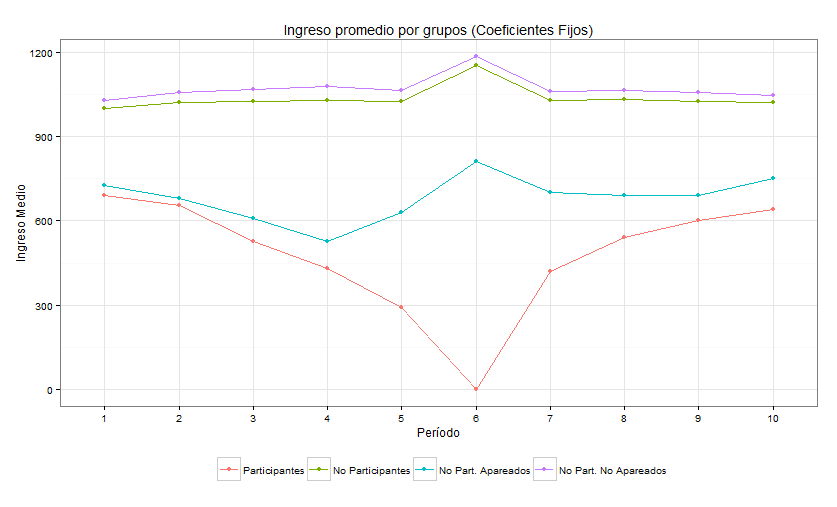
\includegraphics{DipConstant.png}

El gráfico de las distribuciones de los $\theta_{i}$ muestra que éstas
difieren bastante entre participantes y no participantes en el caso de
los coeficientes comunes.

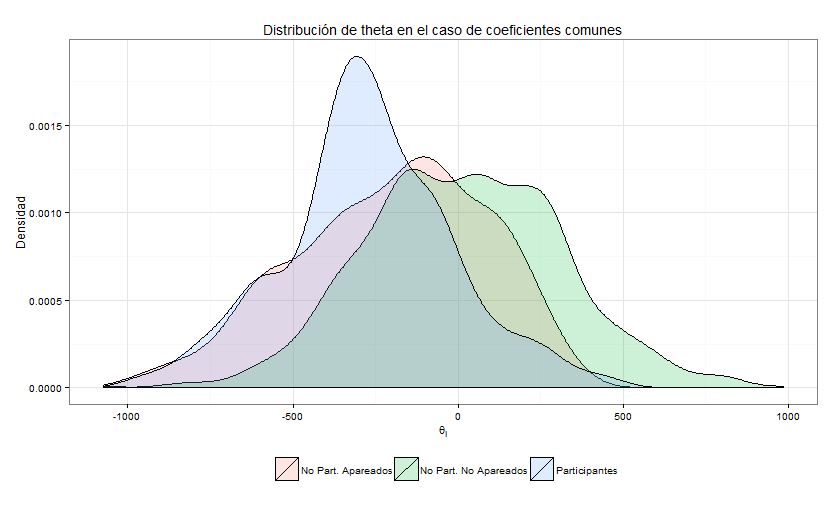
\includegraphics{ThetaConst.png}

Para el caso de coeficientes aleatorios se observa que los resultados
son muy diferentes:

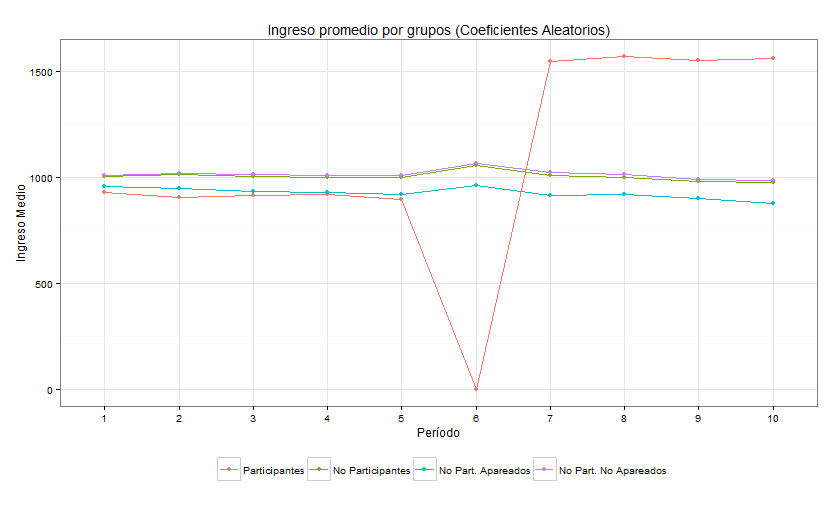
\includegraphics{DipRandom.png}

La figura del ingreso promedio para cada período difiere notablemente de
la obtenida por Heckman et Al. (Fig. 15, pág. 2023) porque se observa un
salto de gran magnitud en los ingresos del grupo tratado a partir del
período 7, debido a la magnitud de $alpha_{i}$.

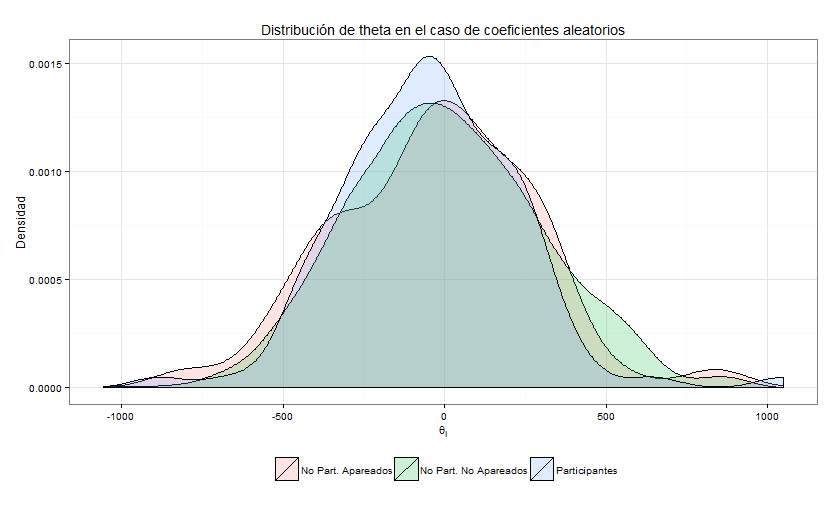
\includegraphics{ThetaRand.png}

Como contracara de lo anterior, las distribuciones de los distintos
subgrupos en el caso de los coeficientes aleatorios son muy similares,
reflejando con mucha exactitud los resultados de Heckman.

Resumiendo, la diferencia entre el caso de coeficientes fijos y el de
coeficientes aleatorios reside en el mecanismo de seleccíon, porque en
el segundo sólo dependerá de $\theta_{i}$ y de $U_{it}$ ya que la
ganancia de participar es igual para todos ya que $\alpha$ es idéntico
para todos los individuos, y es ésta autoselección la que se refleja en
el ``dip'' mas pronunciado para éste caso.

\section{Simulación de montecarlo}\label{simulacion-de-montecarlo}

La simulación de montecarlo es un método de simulación que se basa en
remuestreos repetidos de la misma población, en este caso se basa en
generar 100 muestras de 1000 individuos a los cuales se les estiman un
conjunto de estimadores que se detallarán a continuación.

\subsection{Estimador ``Cross-section''}\label{estimador-cross-section}

Este estimador se basa en comparar las medias de ingresos entre
participantes y no participantes en el momento $t$, en este caso se
escogen cuatro momentos: $k+1$, $k+2$, $k+3$ y $k+4$.

Siguiendo a (Heckman, Lalonde, and Smith 1999, 1986), éste estimador no
comapra a la misma persona ya que ésta no puede pertenecer
simultáneamente a los grupos de control y de tratamiento, sino que lo
hace invocando un supuesto de identificación adicional:

\[ E(Y_{0t}/D=1)=E(Y_{0t}/D=0) \]

Esto es, que las personas que no participan del programa poseen el mismo
resultado sin tratamiento que los que participan. Si éste supuesto es
válido, el estimador de corte transversal es:

\[ \left(\overline{Y}_{1t}\right)_{1}-\left(\overline{Y}_{0t}\right)_{0} \]

Y es válido bajo el supuesto de identificación porque:

\[ E\left[\left(\overline{Y}_{1t}\right)_{1}-\left(\overline{Y}_{0t}\right)_{0}\right]=E(\Delta_{t}/D=1) \]

La implementación consiste en calcular una regresión simple por Mínimos
Cuadrados Ordinarios de $Y_{it}$ en $D_{i}$ para cada período. Comom
primer lugar se obtiene la submuestra de individuos apareados a partir
de la variable \texttt{partc}, una dummy igual a 1 si el individuo $i$
del grupo de control fue matcheado con otro del grupo de tratamiento y 0
en caso contrario. Luego se repiten las estimaciones, primero para toda
la población y luego sólo para el grupo apareado (igual a los 100
individuos del grupo de tratamiento más sus contrapartes apareadas en el
grupo de control).

El comando \texttt{lm} realiza una regresión lineal entre \texttt{y\_t}
y \texttt{D\_i} y garda los resultdos en la variable \texttt{regci}
$(i=1, 2, 3, 4)$, con el comando \texttt{summary} se obtiene el valor
del coeficiente de la variable \texttt{D\_i}. Por último se utiliza el
comando \texttt{vcovHC} para estimar los errores estandar robustos a
heterocedasticidad y autocorrelación (Zeileis 2006), la opción
\texttt{type="HC1"} se agrega para que el resultado sea similar al
comando \texttt{robust} de Stata e indica la forma que deberá tener la
matriz de White, En este caso no es otra cosa que una corrección por
grados de libertad de dicha matriz, si $e_{i}$ son los errores de la
regresión y $\mathbf{X}$ es la matriz de regresores, éste estimador de
la matriz de covarianzas será:

\[ HC1=\frac{N}{N-k}(\mathbf{X}'\mathbf{X})^{-1}\mathbf{X}diag[e_{i}^{2}]\mathbf{X}(\mathbf{X}'\mathbf{X})^{-1}=\frac{N}{N-k}HC0 \]

Por último, con el comando \texttt{coeftest} se obtienen los valores de
los mencionados errores estándar.

\begin{Shaded}
\begin{Highlighting}[]
\NormalTok{matched<-}\KeywordTok{subset}\NormalTok{(dat, partc==}\DecValTok{1}\NormalTok{)}

\CommentTok{#Periodo k+1}
\KeywordTok{library}\NormalTok{(sandwich)}
\KeywordTok{library}\NormalTok{(lmtest)}

\CommentTok{#Total de la población}
\NormalTok{regc1<-}\KeywordTok{lm}\NormalTok{(y_7~D_i, }\DataTypeTok{data=}\NormalTok{dat)}
\NormalTok{alfa_cs1<-}\KeywordTok{summary}\NormalTok{(regc1)$coefficients[}\DecValTok{2}\NormalTok{,}\DecValTok{1}\NormalTok{]}
\NormalTok{regc1$newse<-}\KeywordTok{vcovHC}\NormalTok{(regc1, }\DataTypeTok{type=}\StringTok{"HC1"}\NormalTok{)}
\NormalTok{se_cs1<-}\KeywordTok{coeftest}\NormalTok{(regc1,regc1$newse)[}\DecValTok{2}\NormalTok{,}\DecValTok{2}\NormalTok{]}

\CommentTok{#Grupo apareado}
\NormalTok{regc1m<-}\KeywordTok{lm}\NormalTok{(y_7~D_i, }\DataTypeTok{data=}\NormalTok{matched)}
\NormalTok{alfa_cs1m<-}\KeywordTok{summary}\NormalTok{(regc1m)$coefficients[}\DecValTok{2}\NormalTok{,}\DecValTok{1}\NormalTok{]}
\NormalTok{regc1m$newse<-}\KeywordTok{vcovHC}\NormalTok{(regc1m, }\DataTypeTok{type=}\StringTok{"HC1"}\NormalTok{)}
\NormalTok{se_cs1m<-}\KeywordTok{coeftest}\NormalTok{(regc1m,regc1m$newse)[}\DecValTok{2}\NormalTok{,}\DecValTok{2}\NormalTok{]}

\CommentTok{#Periodo k+2}
\CommentTok{#Total de la población}
\NormalTok{regc2<-}\KeywordTok{lm}\NormalTok{(y_8~D_i, }\DataTypeTok{data=}\NormalTok{dat)}
\NormalTok{alfa_cs2<-}\KeywordTok{summary}\NormalTok{(regc2)$coefficients[}\DecValTok{2}\NormalTok{,}\DecValTok{1}\NormalTok{]}
\NormalTok{regc2$newse<-}\KeywordTok{vcovHC}\NormalTok{(regc2, }\DataTypeTok{type=}\StringTok{"HC1"}\NormalTok{)}
\NormalTok{se_cs2<-}\KeywordTok{coeftest}\NormalTok{(regc2,regc2$newse)[}\DecValTok{2}\NormalTok{,}\DecValTok{2}\NormalTok{]}

\CommentTok{#Grupo apareado}
\NormalTok{regc2m<-}\KeywordTok{lm}\NormalTok{(y_8~D_i, }\DataTypeTok{data=}\NormalTok{matched)}
\NormalTok{alfa_cs2m<-}\KeywordTok{summary}\NormalTok{(regc2m)$coefficients[}\DecValTok{2}\NormalTok{,}\DecValTok{1}\NormalTok{]}
\NormalTok{regc2m$newse<-}\KeywordTok{vcovHC}\NormalTok{(regc2m, }\DataTypeTok{type=}\StringTok{"HC1"}\NormalTok{)}
\NormalTok{se_cs2m<-}\KeywordTok{coeftest}\NormalTok{(regc2m,regc2m$newse)[}\DecValTok{2}\NormalTok{,}\DecValTok{2}\NormalTok{]}

\CommentTok{#Periodo k+3}
\CommentTok{#Total de la población}
\NormalTok{regc3<-}\KeywordTok{lm}\NormalTok{(y_9~D_i, }\DataTypeTok{data=}\NormalTok{dat)}
\NormalTok{alfa_cs3<-}\KeywordTok{summary}\NormalTok{(regc3)$coefficients[}\DecValTok{2}\NormalTok{,}\DecValTok{1}\NormalTok{]}
\NormalTok{regc3$newse<-}\KeywordTok{vcovHC}\NormalTok{(regc3, }\DataTypeTok{type=}\StringTok{"HC1"}\NormalTok{)}
\NormalTok{se_cs3<-}\KeywordTok{coeftest}\NormalTok{(regc3,regc1$newse)[}\DecValTok{2}\NormalTok{,}\DecValTok{2}\NormalTok{]}

\CommentTok{#Grupo apareado}
\NormalTok{regc3m<-}\KeywordTok{lm}\NormalTok{(y_9~D_i, }\DataTypeTok{data=}\NormalTok{matched)}
\NormalTok{alfa_cs3m<-}\KeywordTok{summary}\NormalTok{(regc3m)$coefficients[}\DecValTok{2}\NormalTok{,}\DecValTok{1}\NormalTok{]}
\NormalTok{regc3m$newse<-}\KeywordTok{vcovHC}\NormalTok{(regc3m, }\DataTypeTok{type=}\StringTok{"HC1"}\NormalTok{)}
\NormalTok{se_cs3m<-}\KeywordTok{coeftest}\NormalTok{(regc3m,regc3m$newse)[}\DecValTok{2}\NormalTok{,}\DecValTok{2}\NormalTok{]}

\CommentTok{#Periodo k+4}
\CommentTok{#Total de la población}
\NormalTok{regc4<-}\KeywordTok{lm}\NormalTok{(y_10~D_i, }\DataTypeTok{data=}\NormalTok{dat)}
\NormalTok{alfa_cs4<-}\KeywordTok{summary}\NormalTok{(regc4)$coefficients[}\DecValTok{2}\NormalTok{,}\DecValTok{1}\NormalTok{]}
\NormalTok{regc4$newse<-}\KeywordTok{vcovHC}\NormalTok{(regc4, }\DataTypeTok{type=}\StringTok{"HC1"}\NormalTok{)}
\NormalTok{se_cs4<-}\KeywordTok{coeftest}\NormalTok{(regc4,regc4$newse)[}\DecValTok{2}\NormalTok{,}\DecValTok{2}\NormalTok{]}

\CommentTok{#Grupo apareado}
\NormalTok{regc4m<-}\KeywordTok{lm}\NormalTok{(y_10~D_i, }\DataTypeTok{data=}\NormalTok{matched)}
\NormalTok{alfa_cs4m<-}\KeywordTok{summary}\NormalTok{(regc4m)$coefficients[}\DecValTok{2}\NormalTok{,}\DecValTok{1}\NormalTok{]}
\NormalTok{regc4m$newse<-}\KeywordTok{vcovHC}\NormalTok{(regc4m, }\DataTypeTok{type=}\StringTok{"HC1"}\NormalTok{)}
\NormalTok{se_cs4m<-}\KeywordTok{coeftest}\NormalTok{(regc4m,regc4m$newse)[}\DecValTok{2}\NormalTok{,}\DecValTok{2}\NormalTok{]}
\end{Highlighting}
\end{Shaded}

\subsection{Estimador de
Diferencias-en-diferencias}\label{estimador-de-diferencias-en-diferencias}

En este caso es posible utilizar el estimador de DiD dada la estructura
de los datos simulados, ya que se trata de observaciones repetidas de
los mismos individuos, si además, el cambio medio en las observaciones
anterior a la aplicación del programa es idéntico para los grupos de
control y de tratamiento, esto es, si:

\[ E(Y_{0t}-Y_{0t'}/D=1)=E(Y_{0t}-Y_{0t'}/D=0) \]

El estimador de DiD estará dado por:
$\left(\overline{Y}_{1t}-\overline{Y}_{0t'}\right)_{1}-\left(\overline{Y}_{1t}-\overline{Y}_{0t'}\right)_{0}$
para $t>k>t'$.

El estimador se implementa de la siguiente forma, primero se calculan
las diferencias entre los períodos de tiempo deseados y luego se calcula
el estimador, haciendo una corrección por efectos fijos, para lo que se
genera una variable identificadora \texttt{id} que permite
individualizar a cada persona en la muestra y puede utilizarse para
calcular los errores estándar con efectos fijos, para ello se utiliza el
comando \texttt{felm} (fixed effects linear model)\footnote{Este
  estimador implementa la metodología de (Cameron, Gelbach, and Miller
  2011), aunque aquí se lo utiliza a fines de tener en cuenta los
  efectos fijos por individuo únicamente.} y se utilzia como variable de
agrupación al identificador mencionado, el procedimiento para obtener
tanto los estimadores como los efectos fijos es el mismo que para el
caso anterior.

\begin{Shaded}
\begin{Highlighting}[]
\KeywordTok{library}\NormalTok{(lfe)}
\NormalTok{id<-}\KeywordTok{seq}\NormalTok{(}\DecValTok{1}\NormalTok{,n,}\DecValTok{1}\NormalTok{)}
\NormalTok{dat<-}\KeywordTok{cbind}\NormalTok{(id,dat)}
\NormalTok{matched<-}\KeywordTok{subset}\NormalTok{(dat, partc==}\DecValTok{1}\NormalTok{)}

\CommentTok{#Periodo k+3 y k-1}
\CommentTok{#Total de la población}
\NormalTok{Yit_31<-dat$y_9-dat$y_5}
\NormalTok{regdd1<-}\KeywordTok{felm}\NormalTok{(Yit_31~D_i, }\DataTypeTok{clustervar=}\NormalTok{id, }\DataTypeTok{data=}\NormalTok{dat)}
\NormalTok{alfa_dd1<-}\KeywordTok{summary}\NormalTok{(regdd1)$coefficients[}\DecValTok{2}\NormalTok{,}\DecValTok{1}\NormalTok{]}
\NormalTok{se_dd1<-}\KeywordTok{summary}\NormalTok{(regdd1)$coefficients[}\DecValTok{2}\NormalTok{,}\DecValTok{2}\NormalTok{]}

\CommentTok{#Grupo apareado}
\NormalTok{Yit_31<-matched$y_9-matched$y_5}
\NormalTok{regdd1m<-}\KeywordTok{felm}\NormalTok{(Yit_31~D_i, }\DataTypeTok{clustervar=}\NormalTok{matched$id, }\DataTypeTok{data=}\NormalTok{matched)}
\NormalTok{alfa_dd1m<-}\KeywordTok{summary}\NormalTok{(regdd1m)$coefficients[}\DecValTok{2}\NormalTok{,}\DecValTok{1}\NormalTok{]}
\NormalTok{se_dd1m<-}\KeywordTok{summary}\NormalTok{(regdd1m)$coefficients[}\DecValTok{2}\NormalTok{,}\DecValTok{2}\NormalTok{]}

\CommentTok{#Periodo k+3 y k-3}
\CommentTok{#Total de la población}
\NormalTok{Yit_33<-dat$y_9-dat$y_3}
\NormalTok{regdd3<-}\KeywordTok{felm}\NormalTok{(Yit_33~D_i, }\DataTypeTok{clustervar=}\NormalTok{id, }\DataTypeTok{data=}\NormalTok{dat)}
\NormalTok{alfa_dd3<-}\KeywordTok{summary}\NormalTok{(regdd3)$coefficients[}\DecValTok{2}\NormalTok{,}\DecValTok{1}\NormalTok{]}
\NormalTok{se_dd3<-}\KeywordTok{summary}\NormalTok{(regdd3)$coefficients[}\DecValTok{2}\NormalTok{,}\DecValTok{2}\NormalTok{]}

\CommentTok{#Grupo apareado}
\NormalTok{Yit_33<-matched$y_9-matched$y_3}
\NormalTok{regdd3m<-}\KeywordTok{felm}\NormalTok{(Yit_33~D_i, }\DataTypeTok{clustervar=}\NormalTok{matched$id, }\DataTypeTok{data=}\NormalTok{matched)}
\NormalTok{alfa_dd3m<-}\KeywordTok{summary}\NormalTok{(regdd3m)$coefficients[}\DecValTok{2}\NormalTok{,}\DecValTok{1}\NormalTok{]}
\NormalTok{se_dd3m<-}\KeywordTok{summary}\NormalTok{(regdd3m)$coefficients[}\DecValTok{2}\NormalTok{,}\DecValTok{2}\NormalTok{]}

\CommentTok{#Periodo k+3 y k-5}
\CommentTok{#Total de la población}
\NormalTok{Yit_35<-dat$y_9-dat$y_1}
\NormalTok{regdd5<-}\KeywordTok{felm}\NormalTok{(Yit_35~D_i, }\DataTypeTok{clustervar=}\NormalTok{id, }\DataTypeTok{data=}\NormalTok{dat)}
\NormalTok{alfa_dd5<-}\KeywordTok{summary}\NormalTok{(regdd5)$coefficients[}\DecValTok{2}\NormalTok{,}\DecValTok{1}\NormalTok{]}
\NormalTok{se_dd5<-}\KeywordTok{summary}\NormalTok{(regdd5)$coefficients[}\DecValTok{2}\NormalTok{,}\DecValTok{2}\NormalTok{]}

\CommentTok{#Grupo apareado}
\NormalTok{Yit_35<-matched$y_9-matched$y_1}
\NormalTok{regdd5m<-}\KeywordTok{felm}\NormalTok{(Yit_35~D_i, }\DataTypeTok{clustervar=}\NormalTok{matched$id, }\DataTypeTok{data=}\NormalTok{matched)}
\NormalTok{alfa_dd5m<-}\KeywordTok{summary}\NormalTok{(regdd5m)$coefficients[}\DecValTok{2}\NormalTok{,}\DecValTok{1}\NormalTok{]}
\NormalTok{se_dd5m<-}\KeywordTok{summary}\NormalTok{(regdd5m)$coefficients[}\DecValTok{2}\NormalTok{,}\DecValTok{2}\NormalTok{]}
\end{Highlighting}
\end{Shaded}

\subsection{Estimador de Variables
Instrumentales}\label{estimador-de-variables-instrumentales}

\begin{Shaded}
\begin{Highlighting}[]
\CommentTok{#Cargar libreria para estimar VI}
\KeywordTok{library}\NormalTok{(AER)}

\CommentTok{#Primera etapa}
\NormalTok{reg1e<-}\KeywordTok{lm}\NormalTok{(D_i~Z_i)}
\NormalTok{corDZ<-}\KeywordTok{summary}\NormalTok{(reg1e)$coefficients[}\DecValTok{2}\NormalTok{,}\DecValTok{1}\NormalTok{]}
\NormalTok{z<-}\StringTok{ }\KeywordTok{summary}\NormalTok{(reg1e)$coefficients[}\DecValTok{2}\NormalTok{,}\DecValTok{1}\NormalTok{]/}\KeywordTok{summary}\NormalTok{(reg1e)$coefficients[}\DecValTok{2}\NormalTok{,}\DecValTok{2}\NormalTok{]}
\NormalTok{p<-}\DecValTok{2}\NormalTok{*}\KeywordTok{dnorm}\NormalTok{(-}\KeywordTok{abs}\NormalTok{(z))}

\NormalTok{dat<-}\KeywordTok{cbind}\NormalTok{(dat,Z_i)}
\NormalTok{matched<-}\KeywordTok{subset}\NormalTok{(dat, partc==}\DecValTok{1}\NormalTok{)}

\CommentTok{#Periodo k+1}
\CommentTok{#Total de la población}
\NormalTok{regiv1<-}\KeywordTok{ivreg}\NormalTok{(y_7~D_i|Z_i, }\DataTypeTok{data=}\NormalTok{dat)}
\NormalTok{alfa_iv1<-}\KeywordTok{summary}\NormalTok{(regiv1)$coefficients[}\DecValTok{2}\NormalTok{,}\DecValTok{1}\NormalTok{]}
\NormalTok{se_iv1<-}\KeywordTok{summary}\NormalTok{(regiv1)$coefficients[}\DecValTok{2}\NormalTok{,}\DecValTok{2}\NormalTok{]}

\CommentTok{#Grupo apareado}
\NormalTok{regiv1m<-}\KeywordTok{ivreg}\NormalTok{(y_7~D_i|Z_i, }\DataTypeTok{data=}\NormalTok{matched)}
\NormalTok{alfa_iv1m<-}\KeywordTok{summary}\NormalTok{(regiv1m)$coefficients[}\DecValTok{2}\NormalTok{,}\DecValTok{1}\NormalTok{]}
\NormalTok{se_iv1m<-}\KeywordTok{summary}\NormalTok{(regiv1m)$coefficients[}\DecValTok{2}\NormalTok{,}\DecValTok{2}\NormalTok{]}

\CommentTok{#Periodo k+2}
\CommentTok{#Total de la población}
\NormalTok{regiv2<-}\KeywordTok{ivreg}\NormalTok{(y_8~D_i|Z_i, }\DataTypeTok{data=}\NormalTok{dat)}
\NormalTok{alfa_iv2<-}\KeywordTok{summary}\NormalTok{(regiv2)$coefficients[}\DecValTok{2}\NormalTok{,}\DecValTok{1}\NormalTok{]}
\NormalTok{se_iv2<-}\KeywordTok{summary}\NormalTok{(regiv2)$coefficients[}\DecValTok{2}\NormalTok{,}\DecValTok{2}\NormalTok{]}

\CommentTok{#Grupo apareado}
\NormalTok{regiv2m<-}\KeywordTok{ivreg}\NormalTok{(y_8~D_i|Z_i, }\DataTypeTok{data=}\NormalTok{matched)}
\NormalTok{alfa_iv2m<-}\KeywordTok{summary}\NormalTok{(regiv2m)$coefficients[}\DecValTok{2}\NormalTok{,}\DecValTok{1}\NormalTok{]}
\NormalTok{se_iv2m<-}\KeywordTok{summary}\NormalTok{(regiv2m)$coefficients[}\DecValTok{2}\NormalTok{,}\DecValTok{2}\NormalTok{]}

\CommentTok{#Periodo k+3}
\CommentTok{#Total de la población}
\NormalTok{regiv3<-}\KeywordTok{ivreg}\NormalTok{(y_9~D_i|Z_i, }\DataTypeTok{data=}\NormalTok{dat)}
\NormalTok{alfa_iv3<-}\KeywordTok{summary}\NormalTok{(regiv3)$coefficients[}\DecValTok{2}\NormalTok{,}\DecValTok{1}\NormalTok{]}
\NormalTok{se_iv3<-}\KeywordTok{summary}\NormalTok{(regiv3)$coefficients[}\DecValTok{2}\NormalTok{,}\DecValTok{2}\NormalTok{]}

\CommentTok{#Grupo apareado}
\NormalTok{regiv3m<-}\KeywordTok{ivreg}\NormalTok{(y_9~D_i|Z_i, }\DataTypeTok{data=}\NormalTok{matched)}
\NormalTok{alfa_iv3m<-}\KeywordTok{summary}\NormalTok{(regiv3m)$coefficients[}\DecValTok{2}\NormalTok{,}\DecValTok{1}\NormalTok{]}
\NormalTok{se_iv3m<-}\KeywordTok{summary}\NormalTok{(regiv3m)$coefficients[}\DecValTok{2}\NormalTok{,}\DecValTok{2}\NormalTok{]}

\CommentTok{#Periodo k+4}
\CommentTok{#Total de la población}
\NormalTok{regiv4<-}\KeywordTok{ivreg}\NormalTok{(y_10~D_i|Z_i, }\DataTypeTok{data=}\NormalTok{dat)}
\NormalTok{alfa_iv4<-}\KeywordTok{summary}\NormalTok{(regiv4)$coefficients[}\DecValTok{2}\NormalTok{,}\DecValTok{1}\NormalTok{]}
\NormalTok{se_iv4<-}\KeywordTok{summary}\NormalTok{(regiv4)$coefficients[}\DecValTok{2}\NormalTok{,}\DecValTok{2}\NormalTok{]}

\CommentTok{#Grupo apareado}
\NormalTok{regiv4m<-}\KeywordTok{ivreg}\NormalTok{(y_10~D_i|Z_i, }\DataTypeTok{data=}\NormalTok{matched)}
\NormalTok{alfa_iv4m<-}\KeywordTok{summary}\NormalTok{(regiv4m)$coefficients[}\DecValTok{2}\NormalTok{,}\DecValTok{1}\NormalTok{]}
\NormalTok{se_iv4m<-}\KeywordTok{summary}\NormalTok{(regiv4m)$coefficients[}\DecValTok{2}\NormalTok{,}\DecValTok{2}\NormalTok{]}
\end{Highlighting}
\end{Shaded}

\newpage

\section{References}\label{references}

Ashenfelter, Orley. 1978. ``Estimating the Effect of Training Programs
on Earnings.'' \emph{Review of Economics and Statistics} 6 (1): 47--57.

Cameron, A. Colin, Jonah B. Gelbach, and Douglas L. Miller. 2011.
``Robust Inference with Multiway Clustering.'' \emph{Journal of Business
and Economic Statistics} 29 (2): 238--249.
doi:\href{http://dx.doi.org/10.1198/jbes.2010.07136}{10.1198/jbes.2010.07136}.
\url{http://dx.doi.org/10.1198/jbes.2010.07136}.

Heckman, James, Robert Lalonde, and Jeffrey Smith. 1999. ``The Economics
and Econometrics of Active Labor Market Programs.'' In \emph{Handbook of
Labor Economics}, edited by Orley Ashenfelter and David Card,
3A:1865--2097. Elsevier Science Publishers.

Ho, Daniel, Kosuke Imai, Gary King, and Elizabeth Stuart. 2011.
``MatchIt: Nonparametric Processing for Parametric Causal Inference.''
\emph{Journal of Statistical Software} 42 (8): 1--28.

Zeileis, Achim. 2006. ``Object-Oriented Computation of Sandwich
Estimators.'' \emph{Journal of Statistical Software} 16 (9) (August 15):
1--16. \url{http://www.jstatsoft.org/v16/i09}.

\end{document}
